\section{Evaluation of Individual Models} \label{sec:evaluation}

\paragraph{Baseline Models.} \Cref{fig:individual_encs_mix_a2} shows the results on Czech$\leftrightarrow$English data averaged from both directions. Different models have different spans of their scores, and therefore it is much harder to select the single best $\alpha$. The most basic model, $M_1$, achieves the best performance (AER = $0.46$). The figure serves as an illustration of the $A_2^\alpha$ landscape.

\begin{figure*}[h!]
    \center
    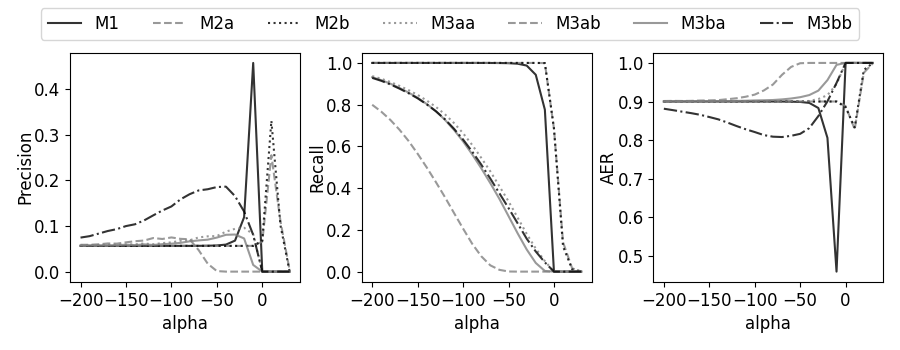
\includegraphics[width=0.92\textwidth]{individual_encs_mix_a2.png}
    \vspace*{-0.3cm}
    \caption{Precision, Recall and AER of individual models on CS$\leftrightarrow$EN data extracted using $A_2$ (directions averaged) \label{fig:individual_encs_mix_a2}}
\end{figure*}

The results on Czech$\leftrightarrow$English data averaged from both directions with $A_3$ can be seen in \Cref{fig:individual_encs_mix_a3}. The case of $\alpha = 0$ corresponds to aligning everything with everything, while $\alpha = 1$ means aligning only the token with the highest score to the single source one (i.e. $A_1$). The different model families behave similarly with respect to Precision, Recall and AER. $M_1$ achieves again the best result (AER = $0.34$), but with a smoother distinction between models.

Out of the model $M_3$ family, $M_3^{bb}$ outperformed the rest significantly. In $A_2$ (\Cref{fig:individual_encs_mix_a2}), the other models, $M_3^{aa}$, $M_3^{ab}$ and $M_3^{ba}$, perform worse than $M_2^a$ and $M_2^b$. This is reversed in case of using the $A_3$ extractor, as shown in \Cref{fig:individual_encs_mix_a3} and \Cref{fig:individual_ende_a3}. For the $M_3$ model family, models with mixed obscuring functions ($M_3^{ab}$ and $M_3^{ba}$) perform worse than with the same obscuring function on both the source and the target side ($M_3^{aa}$ and $M_3^{bb}$).

\begin{figure*}[h!]
    \center
    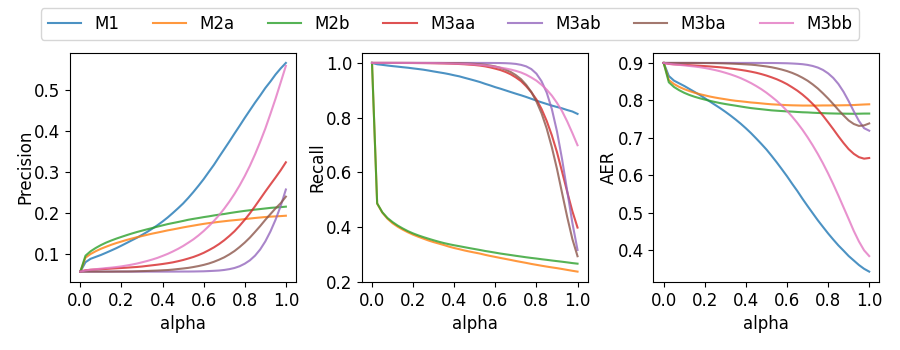
\includegraphics[width=0.93\textwidth]{individual_encs_mix_a3.png}
    \vspace*{-0.4cm}
    \caption{Precision, Recall and AER of individual models on CS$\leftrightarrow$EN extracted using $A_3$ (directions averaged) \label{fig:individual_encs_mix_a3}}
    \vspace*{0.15cm}
\end{figure*}

The English$\rightarrow$German dataset proved to be more difficult. The AER, that are shown in \Cref{fig:individual_ende_a3}, are higher than for Czech$\leftrightarrow$English. The model $M_1$ again achieves the best results with AER = $0.43$. The model ordering is preserved from \Cref{fig:individual_encs_mix_a3}.

\begin{figure*}[h!]
    \center
    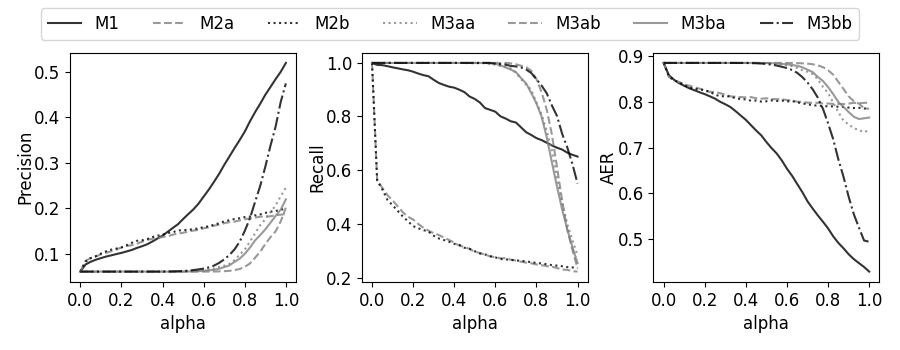
\includegraphics[width=0.93\textwidth]{individual_ende_a3.png}
    \vspace*{-0.4cm}
    \caption{Precision, Recall and AER of individual models on EN$\rightarrow$DE extracted using $A_3$ \label{fig:individual_ende_a3}}
    \vspace*{0.15cm}
\end{figure*}

\Cref{fig:individual_ts_encs_mix_a3} documents that different model types produce different number of alignments per one token. It also shows that the performance rapidly decreases with sentence length. The high AER in \Cref{fig:individual_encs_mix_a3} can be explained by the dataset containing mostly longer sentences (21 tokens on average). The model $M_1$ is still better than $M_3^{bb}$ even on longer sentences despite the fact it does not model the context.

\begin{figure*}[h!]
    \center
    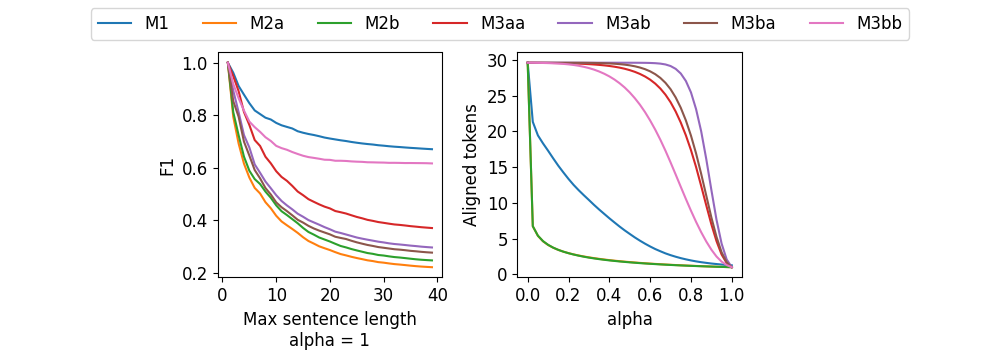
\includegraphics[width=1.0\textwidth]{individual_ts_encs_mix_a3.png}
    \vspace*{-0.4cm}
    \caption{AER for $\alpha=1$ (left) and average number of aligned tokens (right) of individual baseline models on CS$\leftrightarrow$EN extracted using $A_3$ (directions averaged) \label{fig:individual_ts_encs_mix_a3}}
    \vspace*{-0.2cm}
\end{figure*}

The best results were achieved with $A_4^1$ using $M_1$: AER = $0.30$ for German$\rightarrow$English and AER = $0.31$ for Czech$\leftrightarrow$English. The plots (not shown) are very similar to those of $A_3$. Hence $M_3^{bb}$ follows up with AER = $0.38$ and AER = $0.36$ for German and Czech respectively using $A_4^1$.

\begin{table*}[h!]
    \center
    \begin{tabular}{lccc}
        \toprule
        Data & Precision & Recall & AER \\
        \midrule
        Czech$\leftrightarrow$English Small & $0.54$ & $0.66$ & $0.41$ \\
        Czech$\leftrightarrow$English Big & $0.63$ & $0.64$ & $0.38$ \\
        German$\rightarrow$English Small & $0.49$ & $0.55$ & $0.48$\\
        German$\rightarrow$English Small+Big & $0.63$ & $0.72$ & $0.34$ \\
        \bottomrule
    \end{tabular}
    \caption{Precision, Recall and AER of \fastalign{}. Models were evaluated on the respective annotated datasets part. \label{tab:individual_fastalign}}
\end{table*}

\paragraph{\fastalign{}.} For comparison, the results of \fastalign{} can be seen in \Cref{tab:individual_fastalign}. For both language pairs, we use two models, trained on the Small and Big corpora. The motivation for the latter is that the performance of \fastalign{} on 5k sentence pairs is unfairly low in comparison to the other methods because the used MT system has had access to a much larger amount of data. This is shown by the performance difference between these two models.

\begin{table*}[h!]
    \vspace{0.5cm}
    \center
    \begin{tabular}{lcccc}
        \toprule
        Data & Subword Aggregation & Precision & Recall & AER \\
        \midrule
        Czech$\leftrightarrow$English Small & maximum & $0.64$ & $0.81$ & $0.29$ \\
        Czech$\leftrightarrow$English Small & average & $0.64$ & $0.81$ & $0.29$ \\
        German$\rightarrow$English Small\hspace*{-0.5cm}& maximum & $0.69$ & $0.81$ & $0.26$ \\
        German$\rightarrow$English Small\hspace*{-0.5cm}& average & $0.68$ & $0.80$ & $0.27$ \\
        \bottomrule
    \end{tabular}
    \caption{Precision, Recall and AER of attention-based word alignment extracted using $A_3^1$ \label{tab:individual_marian}}
\end{table*}


\paragraph{Attention Scores.} Extracting alignment from MT model attention using $A_3^1$ results in the highest performance (\Cref{tab:individual_marian}). Since the attention scores are between subword units from SentencePiece \citep{kudo2018sentencepiece}, we chose two methods of aggregation to a single score between two tokens (two lists of subwords): (1) taking the maximum probability between two subwords and (2) taking the average probability. They, however, produce almost identical results with respect to the word alignment quality. Scores are listed with $A_3^1$, but $A_2^{0.25}$ achieved very close results.

\begin{table}[h!]
    \vspace{0.5cm}
    \center
    \begin{tabular}{lcccc}
        \toprule
        Model & Method & Precision & Recall & AER \\
        \midrule
        $M_1$ & reverse & $0.56$ & $0.82$ & $0.35$ \\
        $M_1$ & add & $0.59$ & $0.86$ & $0.31$ \\
        $M_1$ & intersect & $0.73$ & $0.77$ & $0.26$ \\
        \midrule
        Attention (avg) & reverse & $0.64$ & $0.81$ & $0.29$ \\
        Attention (avg) & multiply & $0.66$ & $0.83$ & $0.28$ \\
        Attention (avg) & intersect & $0.77$ & $0.70$ & $0.28$ \\
        \bottomrule
    \end{tabular}
    \caption{Average Precision, Recall and AER on Czech$\leftrightarrow$English extracted using $A_4^1$ with symmetrization methods applied for $M_1$ and Attention (avg)\label{tab:individual_symmetry}}
\end{table}

\paragraph{Symmetrization.} Results of symmetrization methods (akin to those described in \Cref{subsec:word_alignment}) for $M_1$ and Attention scores (attention scores aggregated by averaging) are shown in \Cref{tab:individual_symmetry}. Each method is accompanied by an example formula; $p^x$ stands for either $M_1$ or Attention (avg) (in principle any function which produces soft alignments). Similarly, $A_4^1$ could be replaced by other extractors, even though this one worked the best. For \textit{reverse} and \textit{add}, $A_4^1$ is applied on the final result, but for simplicity left out of the formulas.

Method \textit{reverse} consists of using TGT$\rightarrow$SRC translation direction to get alignment scores but then transposing the soft alignment matrix so that the scores are SRC$\rightarrow$TGT.

\vspace*{-0.3cm}
\begin{gather*}
    p_{CS\rightarrow EN}^\text{reverse}(s, t) = p^x_{EN\rightarrow CS}(t, s)
\end{gather*}
\vspace*{0.0cm}

Method \textit{add} simply combines the original and reversed scores before alignments are extracted. The scores of $M_1$ are in log space; therefore, addition is used instead of multiplication. For attentions, multiplication is used, since they are bounded by $[0,1]$.

\vspace*{-0.3cm}
\begin{gather*}
    p_{CS\rightarrow EN}^\text{add}(s, t) = p^x_{CS\rightarrow EN}(s, t)+p^x_{EN\rightarrow CS}(t, s) \\
    p_{CS\rightarrow EN}^\text{mutliply}(s, t) = p^x_{CS\rightarrow EN}(s, t)\cdot p^x_{EN\rightarrow CS}(t, s)\hspace{0.17cm}
\end{gather*}
\vspace*{0.0cm}

Method \textit{intersect} first extracts the alignments for the two directions and then intersects the results (with one direction transposed). This method produces the best results overall (AER = $0.26$), also surpassing $M_1$'s forward direction and attention-based alignments.

\vspace*{-0.3cm}
\begin{gather*}
    A_4^1(p_{CS\rightarrow EN}^\text{intersect}(s, t)) = A_4^1(p^x_{CS\rightarrow EN}(s, t))\cap A_4^1(p^x_{EN\rightarrow CS}(t, s))
\end{gather*}
\vspace*{0.0cm}

In contrast to $M_1$, none of the other models, including attention-based, improved rapidly. This is partly explained by the fact that in other models, the precision-recall balance is shifted from recall to precision, while in $M_1$ it became more balanced after intersection. The reversal also allowed us to get significant results (AER = $0.27$) for the English$\rightarrow$German direction using Attention (avg), for which we did not have an MT system.

\subsection{Extractor Limitations}

Computing word alignments by taking the most probable target token ($A_3^1, A_4^1$) has theoretical limitations to the AER because it makes a faulty assumption that every token is aligned to at least one other token. The Czech$\rightarrow$English dataset has $12\%$ of unaligned tokens and an average of $1.16$ aligned target tokens per source tokens (excluding non-aligned tokens). 

Assuming access to a word alignment oracle ($0$ if not aligned, $1$ if aligned), in case the token is not aligned to any other, all of the scores are $0$. The extractor $A_3^1 = A_1$ will then take all tokens with values equal to the maximum, effectively aligning the in reality unaligned token to every possible one. This extractor is then bound to have maximum recall, but relatively poor accuracy.

The measured performance shows that the $A_2^{\alpha}$ is not the best extraction method. However, it is objectively not prone to this issue because it does not make any assumptions about the number of aligned tokens, and the minimum possible AER is 0 ($A_2^1$ with an oracle). In the next section, we will therefore make use of $A_2^{\alpha_1} \cap A_3^{\alpha_2} \cap A_4^{\alpha_3}$, which provides better performance than individual extractors.